\section{Discussion}

From Background:
\begin{itemize}
	\item It is likely that the thin carpet on concrete and 10~mm double glazed windows will be the cheapest among their counterparts, since they do not absorb sound as well.
	It will be interesting to find out whether the cheapest and ``worst performing" materials in the proposed design solution will meet the privacy requirements of the conference room.
	If they do not, one can then consider using more absorptive (and possibly more expensive) materials.
	\item The arithmetic averages of the reverberation times in the conference room and single office are respectively 0.41~s and 0.40~s.
	Considering that the typical reverberation time of rooms used for speech is between 0.5~s and 1.0~s, these results are a bit low.
	This might be perceived as uncomfortable by the occupants, especially when they and the furnishings will further add absorption and shorten the reverberation times in the rooms.
\end{itemize}

From Q1:
It is interesting to note that the SPLs at 63~Hz and 125~Hz are low relative to the other SPLs.
This is largely because of the high end reflection losses at low frequencies.

From Q2:
According to Table~2.5 in the course notes \citep{unit2}, the recommended NR for an office ranges between 25 and 45.
The conference room's NR of 50 can therefore be seen as a bit high.

From Q3: Comment on Figure~\ref{fig:Lpmale}:
\begin{itemize}
	\item The ductwork attenuated mostly on the lower end of the spectrum (up to 58~dB); this is mostly due to high end reflection losses (c.f. Question 1)
	
	\item The partition is more effective at reducing sound at the higher end of the frequency spectrum (up to 78~dB). This is because L\textsubscript{p\textsubscript{male\textsubscript{2}partition}} varies with R and A\textsubscript{2}, which are both more effective sound level reducers at the higher end of the frequency spectrum.
	\begin{itemize}
		\item The SRI of the partition, R, is independent of the wall or room properties.
		The effectiveness of the partition at reducing sound generally increases with frequency (see R in graph, where it peaks with 64~dB at 2~kHz).
		
		\item A\textsubscript{2} is the sum of surface absorptions in the single office.
		The A\textsubscript{2} curve in the graph resembles the curve of a combined membrane and porous absorber with two peaks (19.7~dB at 125~Hz and 27~dB at 4~kHz).
		The single office thus has slightly more absorption on the higher end of the frequency spectrum.
	\end{itemize}

	\item The sum of the SPLs in the single office basically consists of the peaks of L\textsubscript{p\textsubscript{male\textsubscript{2}ducts}} and L\textsubscript{p\textsubscript{male\textsubscript{2}partition}}.
\end{itemize}

\begin{figure}[htbp]
	\centering
	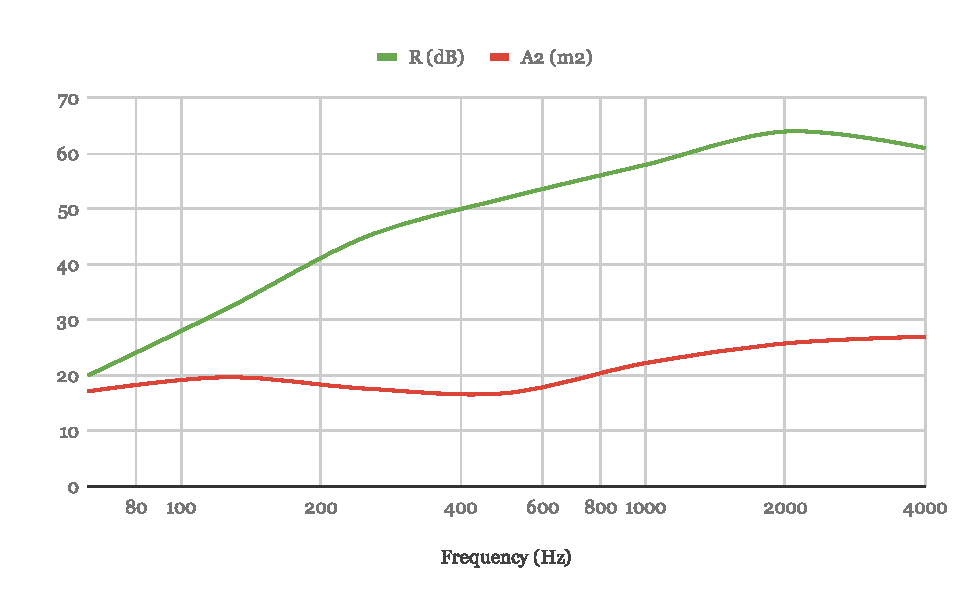
\includegraphics[width=\textwidth]{figures/R+A2.eps}
	\rule{\textwidth}{0.5pt} % use line???
	\caption{The partition's SRI, R, and the single office's total absorption, A\textsubscript{2}.}
	\label{fig:R+A2}
\end{figure}

Suggestions/ improvements?
\begin{itemize}
	\item The carpet's mid-frequency absorption properties can be improved by increasing its thickness
	\item Double glazed windows: Changing the panel mass or the depth of the air space can change the frequency of maximum absorption
	\item Suspended ceiling?
	\item Partition?
\end{itemize}